\section{Exploring the incidents' classification}

\subsection*{Question 4.1}
\textit{Incidents have two types: the type of the incident at the moment it was reported (Initial Type Group) and the type of the incident after it has been studied and classified (Event Clearance Group). Obviously, there should be some kind of correlation of the latter with the former (for instance, incidents reported as robberies are very likely to be also classified finally as robberies). How strong is this correlation?}

The visualization uses a heatmap to show this correlation.
The rows report the incident types at the moment it was reported, while the columns the type it was classified as (we will refer to it as the ``final'' type).
Each cell in the map contains a square, whose area and color are proportional to the number of record for the particular row and column.
Color uses a continuos heat colormap.

The order of rows and columns is initially alphabetical.
However, since there is no $1$-to-$1$ mapping between the categorical values of ``Initial Type Group'' and ``Event Clearance Group'', this order does not have any particular meaning.
Starting from such an order, we have moved some rows and columns to types which seems to be possibly correlated.
For example, ``Initial Type Group'' has the value \textit{Parking Violation}, but ``Event Clearance Group'' does not have it:
we have it closed to \textit{Traffic Related Calls}.

% TODO -> update the picture
\begin{figure}[h]
	\centering
	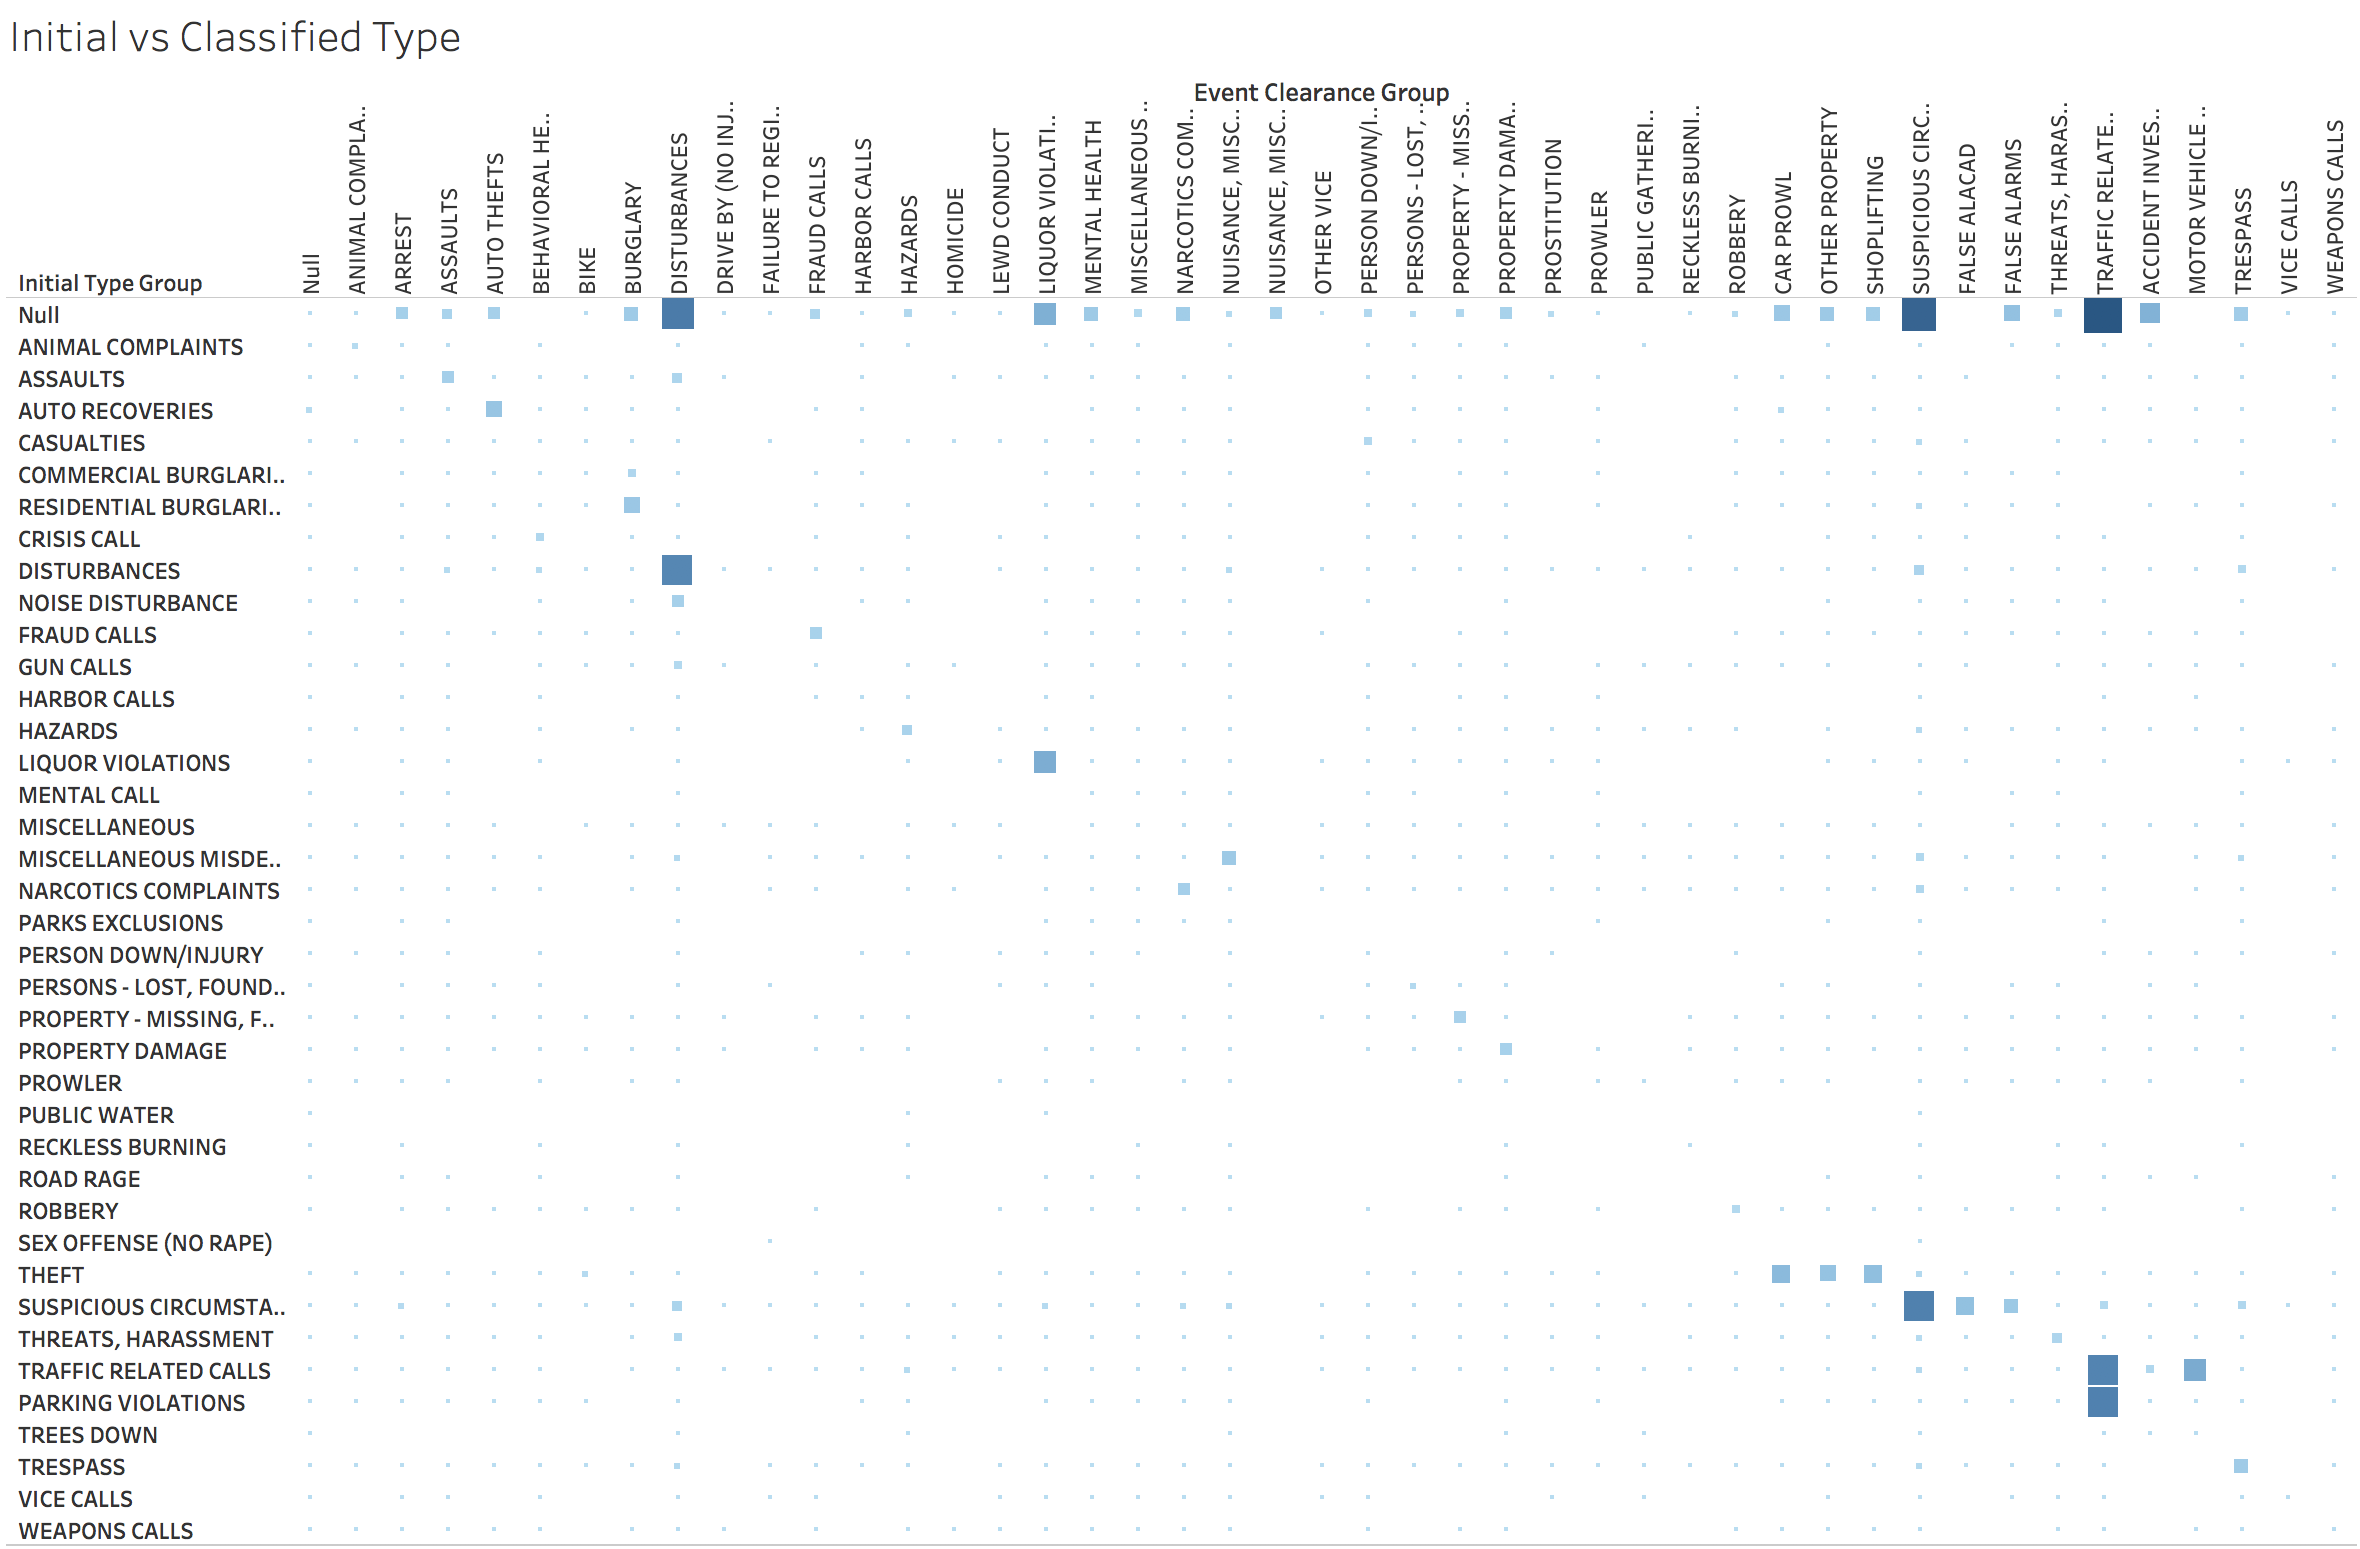
\includegraphics[width=\columnwidth]{figures/4_1_initial_vs_final_group_heatmap}
	\caption{Correlation between the initial and final incident type. The sheet is called ``Initial vs Final Type'' in Tableau.}
	\label{fig:4_1_initial_vs_final_group_heatmap}
\end{figure}

\cref{fig:4_1_initial_vs_final_group_heatmap} show the visualization.
We can see that:
\begin{itemize}
    \item After some reordering of columns, most of the big squares are along the main diagonal. This means there is a very high correlation between the initial and final types of incidents.
    \item In many cases there is a $1$-to-$1$ match between the initial and final type (e.g. \textit{Disturbances}). In some cases a single initial type matches multiple more specific final types (e.g. \textit{Theft} matches with \textit{Car prowl}, \textit{Other property} and \textit{Shoplifting}).
    \item The first row of the table has a different behaviour. This row represent items without an initial type. They matches different final types, mostly \textit{Disturbances}, \textit{Suspicious circumstances} and \textit{Traffic related calls}.
\end{itemize}

To sum up, there seems to be a very high correlation between the initial types and the final types.

\subsection*{Question 4.2}
\textit{How do the total number of incidents break down per incident reported type (Initial Type Group) and incident resolution type (Event Clearance Group)?}


\subsection*{Question 4.3}
\textit{How do the total number of incidents break down per incident resolution type (Event Clearance Group) and incident resolution subtype (Event Clearance Subgroup)?}
